\documentclass[12pt]{article}
\usepackage{amsmath}
\usepackage{tikz}
\begin{document}
\title{Computer Science 181, Homework 3}
\date{April 23rd, 2018}
\author{Michael Wu\\UID: 404751542}
\maketitle

\section*{Postponed Problem 5}

The set of finite state languages is closed under homomorphisms on a language's alphabet \(\Sigma\). Therefore, if \(L_\text{five}\) is a
finite state language, every homomorphism on \(\Sigma=\{a, b, c\}\) results in a finite state language when applied
to \(L_\text{five}\). But the homomorphism
\[h(a)=a \qquad h(b)=b \qquad h(c)=\epsilon\]
yields \(h(L_\text{five})=L_\text{NFS}\), which is not a finite state language. Therefore \(L_\text{five}\) cannot be a finite
state language.

\section*{Problem 0}

The first DFA can be made as shown below.
\begin{center}
        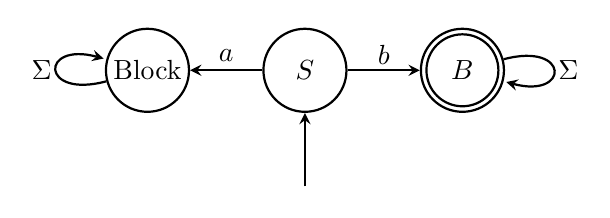
\begin{tikzpicture}
                \begin{scope}[auto, every node/.style={thick, draw,circle,minimum size=3em,inner sep=1}]
                        \node (Bl) at (0,0) {Block};
                        \node (S) at (2,0) {\(S\)};
                        \node (B) at (4,0) {\(B\)};
                        \draw[black, thick] (4,0) circle [radius=1.3em];
                \end{scope}
                \node [draw=none, inner sep=0pt] (I) at (2,-1.5) {};
                \begin{scope}[auto, every node/.style={minimum size=1em,inner sep=1}, every path/.style={thick, ->, >=stealth}]
                        \path (I) edge (S);
                        \path (S) edge node [above] {\(b\)} (B);
                        \path (S) edge node [above] {\(a\)} (Bl);
                        \path (B) edge [loop right] node {\(\Sigma\)} (B);
                        \path (Bl) edge [loop left] node {\(\Sigma\)} (Bl);
               \end{scope}
        \end{tikzpicture}
\end{center}
The second DFA can be made as shown below.
\begin{center}
        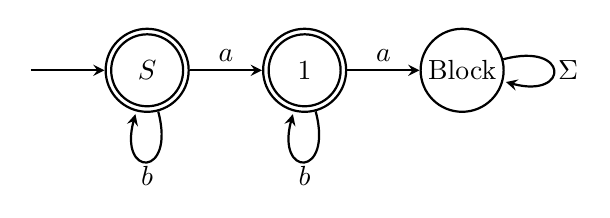
\begin{tikzpicture}
                \begin{scope}[auto, every node/.style={thick, draw,circle,minimum size=3em,inner sep=1}]
                        \node (S) at (0,0) {\(S\)};
                        \draw[black, thick] (0,0) circle [radius=1.3em];
                        \draw[black, thick] (2,0) circle [radius=1.3em];
                        \node (1) at (2,0) {\(1\)};
                        \node (Bl) at (4,0) {Block};
                \end{scope}
                \node [draw=none, inner sep=0pt] (I) at (-1.5,0) {};
                \begin{scope}[auto, every node/.style={minimum size=1em,inner sep=1}, every path/.style={thick, ->, >=stealth}]
                        \path (I) edge (S);
                        \path (S) edge node {\(a\)} (1);
                        \path (S) edge [loop below] node {\(b\)} (S);
                        \path (1) edge node {\(a\)} (Bl);
                        \path (1) edge [loop below] node {\(b\)} (1);
                        \path (Bl) edge [loop right] node {\(\Sigma\)} (Bl);
               \end{scope}
        \end{tikzpicture}
\end{center}
Their intersection should be as shown below.
\begin{center}
        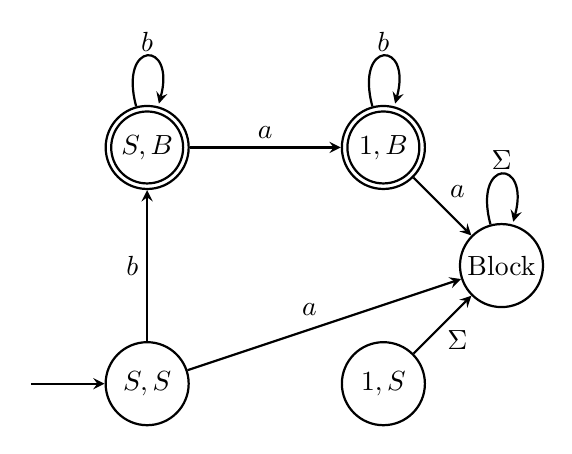
\begin{tikzpicture}
                \begin{scope}[auto, every node/.style={thick, draw,circle,minimum size=3em,inner sep=1}]
                        \node (SS) at (0,0) {\(S,S\)};
                        \node (SB) at (0,3) {\(S,B\)};
                        \draw[black, thick] (0,3) circle [radius=1.3em];
                        \node (1S) at (3,0) {\(1,S\)};
                        \node (1B) at (3,3) {\(1,B\)};
                        \draw[black, thick] (3,3) circle [radius=1.3em];
                        \node (Bl) at (4.5, 1.5) {Block};
                \end{scope}
                \node [draw=none, inner sep=0pt] (I) at (-1.5,0) {};
                \begin{scope}[auto, every node/.style={minimum size=1em,inner sep=1}, every path/.style={thick, ->, >=stealth}]
                        \path (I) edge (SS);
                        \path (SS) edge node {\(b\)} (SB);
                        \path (SB) edge node {\(a\)} (1B);
                        \path (SB) edge [loop above] node {\(b\)} (SB);
                        \path (1B) edge [loop above] node {\(b\)} (1B);
                        \path (SS) edge node {\(a\)} (Bl);
                        \path (1B) edge node {\(a\)} (Bl);
                        \path (Bl) edge [loop above] node {\(\Sigma\)} (Bl);
                        \path (1S) edge node [below right] {\(\Sigma\)} (Bl);
               \end{scope}
        \end{tikzpicture}
\end{center}
Here I have simplified a bit by grouping all blocking states into a single one, as in an intersection if any DFA blocks then their intersection will block.
I also include the useless state \(1,S\) to illustrate the cartesian product of the two DFAs.

\section*{Problem 1}

\paragraph{a)}

A DFA for \(L_\text{one}\) is shown below.
\begin{center}
        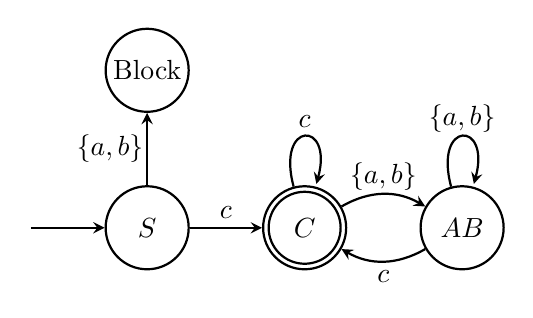
\begin{tikzpicture}
                \begin{scope}[auto, every node/.style={thick, draw,circle,minimum size=3em,inner sep=1}]
                        \node (S) at (0,0) {\(S\)};
                        \node (C) at (2,0) {\(C\)};
                        \draw[black, thick] (2,0) circle [radius=1.3em];
                        \node (AB) at (4,0) {\(AB\)};
                        \node (Bl) at (0,2) {Block};
                \end{scope}
                \node [draw=none, inner sep=0pt] (I) at (-1.5,0) {};
                \begin{scope}[auto, every node/.style={minimum size=1em,inner sep=1}, every path/.style={thick, ->, >=stealth}]
                        \path (I) edge (S);
                        \path (S) edge node {\(c\)} (C);
                        \path (S) edge node {\(\{a,b\}\)} (Bl);
                        \path (C) edge [loop above] node {\(c\)} (C);
                        \path (C) edge [bend left] node {\(\{a,b\}\)} (AB);
                        \path (AB) edge [bend left] node {\(c\)} (C);
                        \path (AB) edge [loop above] node {\(\{a,b\}\)} (AB);
                \end{scope}
        \end{tikzpicture}
\end{center}
The corresponding NFA for \(L_\text{one}^*\) is shown below.
\begin{center}
        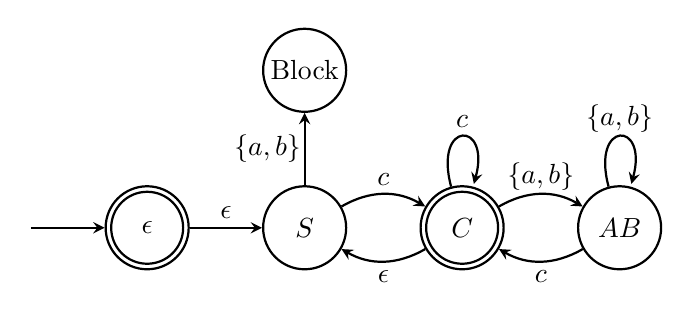
\begin{tikzpicture}
                \begin{scope}[auto, every node/.style={thick, draw,circle,minimum size=3em,inner sep=1}]
                        \node (Ep) at (-2,0) {\(\epsilon\)};
                        \draw[black, thick] (-2,0) circle [radius=1.3em];
                        \node (S) at (0,0) {\(S\)};
                        \node (C) at (2,0) {\(C\)};
                        \draw[black, thick] (2,0) circle [radius=1.3em];
                        \node (AB) at (4,0) {\(AB\)};
                        \node (Bl) at (0,2) {Block};
                \end{scope}
                \node [draw=none, inner sep=0pt] (I) at (-3.5,0) {};
                \begin{scope}[auto, every node/.style={minimum size=1em,inner sep=1}, every path/.style={thick, ->, >=stealth}]
                        \path (I) edge (Ep);
                        \path (Ep) edge node {\(\epsilon\)} (S);
                        \path (S) edge [bend left] node {\(c\)} (C);
                        \path (C) edge [bend left] node {\(\epsilon\)} (S);
                        \path (S) edge node {\(\{a,b\}\)} (Bl);
                        \path (C) edge [loop above] node {\(c\)} (C);
                        \path (C) edge [bend left] node {\(\{a,b\}\)} (AB);
                        \path (AB) edge [bend left] node {\(c\)} (C);
                        \path (AB) edge [loop above] node {\(\{a,b\}\)} (AB);
                \end{scope}
        \end{tikzpicture}
\end{center}

\paragraph{b)}

No they are not the same, as \(L_\text{one}\) does not contain the empty string \(\epsilon\), while \(L_\text{one}^*\) does.

\section*{Problem 2}

\paragraph{a)}

A DFA for \(L_\text{two}\) is shown below.
\begin{center}
        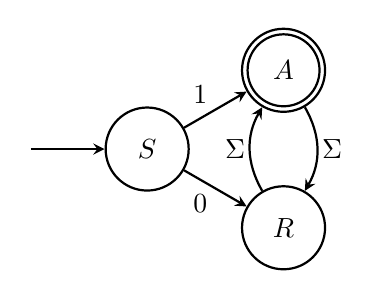
\begin{tikzpicture}
                \begin{scope}[auto, every node/.style={thick, draw,circle,minimum size=3em,inner sep=1}]
                        \node (S) at (0,0) {\(S\)};
                        \node (A) at (1.732,1) {\(A\)};
                        \draw[black, thick] (1.732,1) circle [radius=1.3em];
                        \node (R) at (1.732,-1) {\(R\)};
                \end{scope}
                \node [draw=none, inner sep=0pt] (I) at (-1.5,0) {};
                \begin{scope}[auto, every node/.style={minimum size=1em,inner sep=1}, every path/.style={thick, ->, >=stealth}]
                        \path (I) edge (S);
                        \path (S) edge node {\(1\)} (A);
                        \path (S) edge [below left] node {\(0\)} (R);
                        \path (A) edge [bend left] node {\(\Sigma\)} (R);
                        \path (R) edge [bend left] node {\(\Sigma\)} (A);
                \end{scope}
        \end{tikzpicture}
\end{center}
The corresponding NFA for \(L_\text{two}\cdot L_\text{two}\) is shown below.
\begin{center}
        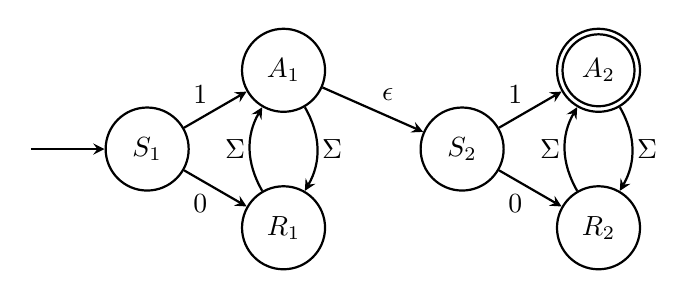
\begin{tikzpicture}
                \begin{scope}[auto, every node/.style={thick, draw,circle,minimum size=3em,inner sep=1}]
                        \node (S) at (0,0) {\(S_1\)};
                        \node (A) at (1.732,1) {\(A_1\)};
                        \node (R) at (1.732,-1) {\(R_1\)};
                        \node (S2) at (4,0) {\(S_2\)};
                        \node (A2) at (5.732,1) {\(A_2\)};
                        \draw[black, thick] (5.732,1) circle [radius=1.3em];
                        \node (R2) at (5.732,-1) {\(R_2\)};
                \end{scope}
                \node [draw=none, inner sep=0pt] (I) at (-1.5,0) {};
                \begin{scope}[auto, every node/.style={minimum size=1em,inner sep=1}, every path/.style={thick, ->, >=stealth}]
                        \path (I) edge (S);
                        \path (S) edge node {\(1\)} (A);
                        \path (S) edge [below left] node {\(0\)} (R);
                        \path (A) edge [bend left] node {\(\Sigma\)} (R);
                        \path (R) edge [bend left] node {\(\Sigma\)} (A);
                        \path (A) edge node {\(\epsilon\)} (S2);
                        \path (S2) edge node {\(1\)} (A2);
                        \path (S2) edge [below left] node {\(0\)} (R2);
                        \path (A2) edge [bend left] node {\(\Sigma\)} (R2);
                        \path (R2) edge [bend left] node {\(\Sigma\)} (A2);
                \end{scope}
        \end{tikzpicture}
\end{center}

\paragraph{b)}

\(L_\text{two}\cdot L_\text{two}\) does not equal \(L_\text{two}\), since \(1\) is in \(L_{two}\) but not in \(L_\text{two}\cdot L_\text{two}\).

\section*{Problem 3}

\[1000^* \cup 0100^* \cup 000^*10^* \cup 000^*\]

\section*{Problem 4}

\paragraph{a)}

\[
        \begin{array}{c|c|c}
                \text{Current State} & \text{Word} & \text{Next State}\\
                \hline
                q_\text{start} & w_1 = ab & q_2\\
                q_2 & w_2 = \epsilon & q_1\\
                q_1 & w_3 = ab & q_1\\
                q_1 & w_4 = aa & q_2\\
                q_2 & w_5 = ba & q_\text{accept}
        \end{array}
\]

\paragraph{b)}

This is false, as the string \(abab\) will be accepted. First \(ab\) will cause a move from \(q_\text{start}\) to \(q_2\), then \(ab\) will cause
a move into \(q_\text{accept}\). This string has more than one \(b\) and an even number of \(a\)'s, proving this statement is false.

\section*{Problem 5}

Assume for contradiction that this language
\[L=\{0^i1^j0^k | i,j,k\geq0 \wedge k=|i-j|\}\]
is finite state. Then by the pumping lemma if a language is finite state then there exists some \(p\) such that for any string \(s\) in
\(L\) with \(|s|>p\), \(s\) can be split into three strings \(x\), \(y\), and \(z\) where \(s=xyz\), \(|y|\geq 1\), \(|xy|\leq p\), and \(xy^*z\subseteq L\).
Take the string \(0^p1^p\in L\), and note that \(xy\) must be a string made entirely of \(0\)'s, since \(|xy|\leq p\). Additionally, \(y\) must be in \(0^+\),
since \(|y|\geq 1\). Let \(x=0^a\) and \(y=0^b\) for some constants \(a\geq 0\) and \(b>0\). Then \(z\) must be \(0^{p-a-b}1^p\). By the pumping lemma \(xy^*z\subseteq L\),
so
\[\{0^a(0^b)^*0^{p-a-b}1^p|a\geq0 \wedge b>0\}\subseteq L\]
This can be stated equivalently as
\[\{0^{p-b}0^{xb}1^p|\forall x\in\{0,1,2,\ldots\} \wedge b>0\}\subseteq L\]
When \(x=2\), this means that the string \(0^{p+b}1^p\in L\) for some constant \(b>0\). But in the definition of \(L\), this string has the parameters
\(i=p+b\), \(j=p\), and \(k=0\). Thus \(k\neq |i-j|\) and \(0^{p+b}1^p\notin L\). This is a contradiction, so \(L\) cannot be finite state.

\end{document}